
%%--------------------------------------------------
%% Halliday: Fundamentals of Physics
%%--------------------------------------------------


%% Chapter 12: Equilibrium and Elasticity
%%--------------------------------------------------


%% Learning Objectives
%%--------------------------------------------------

%% 12.01: Distinguish between equilibrium and static equilibrium.
%% 12.02: Specify the four conditions for static equilibrium.
%% 12.03: Explain center of gravity and how it relates to center of mass.
%% 12.04: For a given distribution of particles, calculate the coordinates of the center of gravity and the center of mass.


%% Halliday Multiple Choice Questions
%%--------------------------------------------------
\element{halliday-mc}{
\begin{question}{halliday-ch12-q01}
    A net torque applied to a rigid object always tends to produce:
    \begin{choices}
        \wrongchoice{linear acceleration}
        \wrongchoice{rotational equilibrium}
      \correctchoice{angular acceleration}
        \wrongchoice{rotational inertia}
        \wrongchoice{none of these}
    \end{choices}
\end{question}
}

\element{halliday-mc}{
\begin{question}{halliday-ch12-q02}
    The conditions that the net force and the net torque both vanish:
    \begin{choices}
      \correctchoice{hold for every rigid body in equilibrium}
        \wrongchoice{hold only for elastic solid bodies in equilibrium}
        \wrongchoice{hold for every solid body}
        \wrongchoice{are always sufficient to calculate the forces on a solid object in equilibrium}
        \wrongchoice{are sufficient to calculate the forces on a solid object in equilibrium only if the object is elastic}
    \end{choices}
\end{question}
}

\element{halliday-mc}{
\begin{question}{halliday-ch12-q03}
    For an object in equilibrium the net torque acting on it vanishes only if each torque is calculated about:
    \begin{choices}
        \wrongchoice{the center of mass}
        \wrongchoice{the center of gravity}
        \wrongchoice{the geometrical center}
        \wrongchoice{the point of application of the force}
      \correctchoice{the same point}
    \end{choices}
\end{question}
}

\element{halliday-mc}{
\begin{question}{halliday-ch12-q04}
    For a body to be in equilibrium under the combined action of several forces:
    \begin{choices}
        \wrongchoice{all the forces must be applied at the same point}
        \wrongchoice{all of the forces form pairs of equal and opposite forces}
      \correctchoice{the sum of the components of all the forces in any direction must equal zero}
        \wrongchoice{any two of these forces must be balanced by a third force}
        \wrongchoice{the lines of action of all the forces must pass through the center of gravity of the body}
    \end{choices}
\end{question}
}

\element{halliday-mc}{
\begin{question}{halliday-ch12-q05}
    For a body to be in equilibrium under the combined action of several forces:
    \begin{choices}
        \wrongchoice{all the forces must be applied at the same point}
        \wrongchoice{all of the forces form pairs of equal and opposite forces}
        \wrongchoice{any two of these forces must be balanced by a third force}
      \correctchoice{the sum of the torques about any point must equal zero}
        \wrongchoice{the lines of action of all the forces must pass through the center of gravity of the body}
    \end{choices}
\end{question}
}

\element{halliday-mc}{
\begin{question}{halliday-ch12-q06}
    To determine if a rigid body is in equilibrium the vector sum of the gravitational forces acting on the particles of the body can be replaced by a single force acting at:
    \begin{choices}
        \wrongchoice{the center of mass}
        \wrongchoice{the geometrical center}
      \correctchoice{the center of gravity}
        \wrongchoice{a point on the boundary}
        \wrongchoice{none of the provided}
    \end{choices}
\end{question}
}

\element{halliday-mc}{
\begin{question}{halliday-ch12-q07}
    The center of gravity coincides with the center of mass:
    \begin{choices}
        \wrongchoice{always}
        \wrongchoice{never}
        \wrongchoice{if the center of mass is at the geometrical center of the body}
      \correctchoice{if the acceleration due to gravity is uniform over the body}
        \wrongchoice{if the body has a uniform distribution of mass}
    \end{choices}
\end{question}
}

\element{halliday-mc}{
\begin{question}{halliday-ch12-q08}
    The location of which of the following points within an object might depend on the orientation of the object?
    \begin{choices}
        \wrongchoice{Its center of mass}
      \correctchoice{Its center of gravity}
        \wrongchoice{Its geometrical center}
        \wrongchoice{Its center of momentum}
        \wrongchoice{None of the provided}
    \end{choices}
\end{question}
}

\element{halliday-mc}{
\begin{question}{halliday-ch12-q09}
    A cylinder placed so it can roll on a horizontal table top,
        with its center of gravity above its geometrical center, is:
    \begin{choices}
        \wrongchoice{in stable equilibrium}
      \correctchoice{in unstable equilibrium}
        \wrongchoice{in neutral equilibrium}
        \wrongchoice{not in equilibrium}
        \wrongchoice{none of the provided}
    \end{choices}
\end{question}
}

\element{halliday-mc}{
\begin{question}{halliday-ch12-q10}
    A cylinder placed so it can roll on a horizontal table top,
        with its center of gravity below its geometrical center, is:
    \begin{choices}
      \correctchoice{in stable equilibrium}
        \wrongchoice{in unstable equilibrium}
        \wrongchoice{in neutral equilibrium}
        \wrongchoice{not in equilibrium}
        \wrongchoice{none of the provided}
    \end{choices}
\end{question}
}

\element{halliday-mc}{
\begin{question}{halliday-ch12-q11}
    A cube balanced with one edge in contact with a table top and with its center of gravity directly equilibrium with respect to rotation about the edge and in above the edge is in equilibrium with respect to rotation about a horizontal axis that is perpendicular to the edge.
    \begin{choices}
        \wrongchoice{stable, stable}
        \wrongchoice{stable, unstable}
      \correctchoice{unstable, stable}
        \wrongchoice{unstable, unstable}
        \wrongchoice{unstable, neutral}
    \end{choices}
\end{question}
}

\newcommand{\hallidayChTwelveQTwelve}{
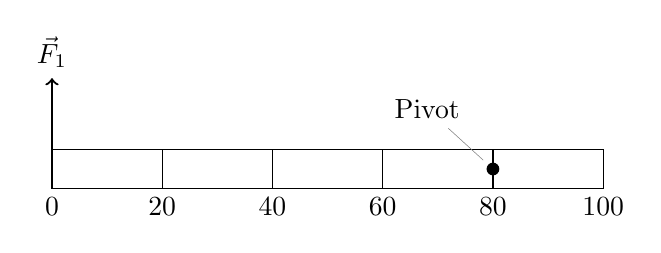
\begin{tikzpicture}[scale=0.7]
    \draw (0,0) rectangle (10cm,2em);
    \foreach \i in {0,20,40,60,80,100}{
        \draw (\i mm,2em) -- (\i mm,0em) node[anchor=north] {\SI{\i}{\centi\meter}};
    }
    %% Pivot
    \draw[fill] (80mm,1em) circle (3pt) node[pin=120:Pivot] {};
    %% Force
    \draw[thick,->] (0,0) -- (0,2cm) node[anchor=south] {$\vec{F}_1$};
\end{tikzpicture}
}

\element{halliday-mc}{
\begin{question}{halliday-ch12-q12}
    A meter stick on a horizontal frictionless table top is pivoted at the \SI{80}{\centi\meter} mark. 
    A force $F_1$ is applied perpendicularly to the end of the stick at \SI{0}{\centi\meter},
        as shown. 
    \begin{center}
        \hallidayChTwelveQTwelve
    \end{center}
    A second force $F_2$ (not shown) is applied perpendicularly at the \SI{100}{\centi\meter} end of the stick. 
    The forces are horizontal. 
    If the stick does not move,
        the force exerted by the pivot on the stick:
    \begin{choices}
        \wrongchoice{must be zero}
        \wrongchoice{must be in the same direction as $F_1$ and have magnitude $|F_2| - |F_1|$}
        \wrongchoice{must be directed opposite to $F_1$ and have magnitude $|F_2| - |F_1|$}
        \wrongchoice{must be in the same direction as $F_1$ and have magnitude $|F_2| + |F_1|$}
      \correctchoice{must be directed opposite to $F_1$ and have magnitude $|F_2| + |F_1|$}
    \end{choices}
\end{question}
}

\element{halliday-mc}{
\begin{question}{halliday-ch12-q13}
    A meter stick on a horizontal frictionless table top is pivoted at the \SI{80}{\centi\meter} mark. 
    A force $F_1$ is applied perpendicularly to the end of the stick at \SI{0}{\centi\meter},
        as shown. 
    \begin{center}
        \hallidayChTwelveQTwelve
    \end{center}
    A second force $F_2$ (not shown) is applied perpendicularly at the \SI{60}{\centi\meter} mark. 
    The forces are horizontal. 
    If the stick does not move,
        the force exerted by the pivot on the stick:
    \begin{choices}
        \wrongchoice{must be zero}
      \correctchoice{must be in the same direction as $F_1$ and have magnitude $|F_2| - |F_1|$}
        \wrongchoice{must be directed opposite to $F_1$ and have magnitude $|F_2| - |F_1|$}
        \wrongchoice{must be in the same direction as $F_1$ and have magnitude $|F_2| + |F_1|$}
        \wrongchoice{must be directed opposite to $F_1$ and have magnitude $|F_2| + |F_1|$}
    \end{choices}
\end{question}
}

\element{halliday-mc}{
\begin{questionmult}{halliday-ch12-q14}
    Three identical uniform rods are each acted on by two or more forces,
        all perpendicular to the rods and all equal in magnitude. 
    Which of the rods could be in static equilibrium if an additional force is applied at the center of mass of the rod?
    \begin{choices}
        \AMCboxDimensions{down=-0.8cm}
        \wrongchoice{
            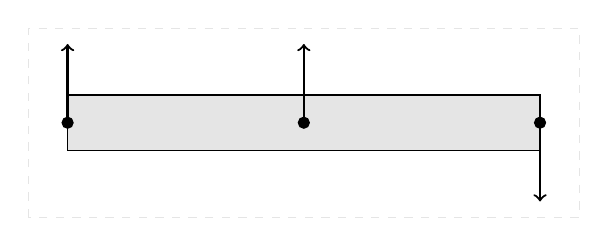
\begin{tikzpicture}
                \draw[white!90!black,dashed] (-0.5,-1.2) rectangle (6.5,1.2);
                \draw[fill=white!90!black] (0,-1em) rectangle (6,1em);
                %% left
                \draw[fill] (0,0em) circle (2pt);
                \draw[thick,->] (0,0em) -- ++(90:1cm);
                %% center
                \draw[fill] (3,0em) circle (2pt);
                \draw[thick,->] (3,0em) -- ++(90:1cm);
                %% right
                \draw[fill] (6,0em) circle (2pt);
                \draw[thick,->] (6,0em) -- ++(270:1cm);
            \end{tikzpicture}
        }
        \wrongchoice{
            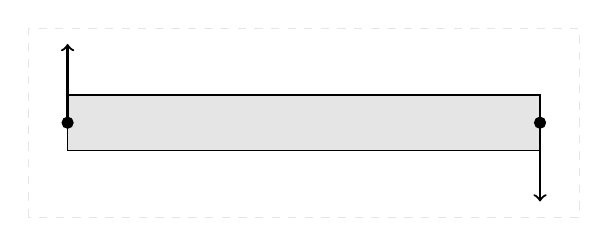
\begin{tikzpicture}
                \draw[white!90!black,dashed] (-0.5,-1.2) rectangle (6.5,1.2);
                \draw[fill=white!90!black] (0,-1em) rectangle (6,1em);
                %% left
                \draw[fill] (0,0em) circle (2pt);
                \draw[thick,->] (0,0em) -- ++(90:1cm);
                %% right
                \draw[fill] (6,0em) circle (2pt);
                \draw[thick,->] (6,0em) -- ++(270:1cm);
            \end{tikzpicture}
        }
        \correctchoice{
            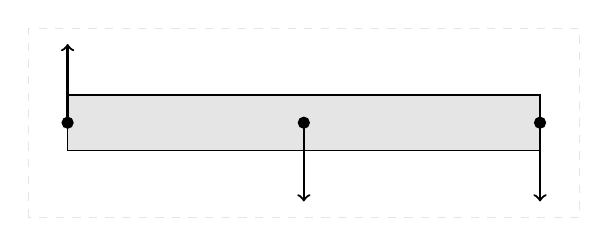
\begin{tikzpicture}
                \draw[white!90!black,dashed] (-0.5,-1.2) rectangle (6.5,1.2);
                \draw[fill=white!90!black] (0,-1em) rectangle (6,1em);
                %% left
                \draw[fill] (0,0em) circle (2pt);
                \draw[thick,->] (0,0em) -- ++(90:1cm);
                %% center
                \draw[fill] (3,0em) circle (2pt);
                \draw[thick,->] (3,0em) -- ++(270:1cm);
                %% right
                \draw[fill] (6,0em) circle (2pt);
                \draw[thick,->] (6,0em) -- ++(270:1cm);
            \end{tikzpicture}
        }
    \end{choices}
\end{questionmult}
}

\element{halliday-mc}{
\begin{question}{halliday-ch12-q15}
    A \SI{160}{\newton} child sits on a light swing and is pulled back and held with a horizontal force of \SI{100}{\newton}.
    The magnitude of the tension force of each of the two supporting ropes is:
    \begin{multicols}{3}
    \begin{choices}
        \wrongchoice{\SI{60}{\newton}}
      \correctchoice{\SI{94}{\newton}}
        \wrongchoice{\SI{120}{\newton}}
        \wrongchoice{\SI{190}{\newton}}
        \wrongchoice{\SI{260}{\newton}}
    \end{choices}
    \end{multicols}
\end{question}
}

\element{halliday-mc}{
\begin{question}{halliday-ch12-q16}
    The diagram shows a stationary \SI{5}{\kilo\gram} uniform rod ($AC$),
        \SI{1}{\meter} long, held against a wall by a rope ($AE$) and friction between the rod and the wall.
    \begin{center}
    \begin{tikzpicture}
        %% Coordinates
        \coordinate (A) at (-6,0);
        \coordinate (B) at (-3,0);
        \coordinate (C) at (0,0);
        \coordinate (D) at (-3,1.5);
        \coordinate (E) at (0,3);
        %% Line
        \node[draw,fill=white!80!black,minimum width=6cm,minimum height=0.1cm] at (B) {};
        \draw (A) -- (D) -- (E);
        %% Nodes
        \draw[fill] (A) circle (1.5pt) node[anchor=north,yshift=-0.1cm] {$A$};
        \draw[fill] (B) circle (1.5pt) node[anchor=north,yshift=-0.1cm] {$B$};
        \draw[fill] (C) circle (1.5pt) node[anchor=north east,yshift=-0.1cm] {$C$};
        \draw[fill] (D) circle (1.5pt) node[anchor=south east] {$D$};
        \draw[fill] (E) circle (1.5pt) node[anchor=south east] {$E$};
        %% Wall
        \node[anchor=west,fill,pattern=north east lines,minimum width=0.1cm, minimum height=5cm] at (0,1.5) {};
        \draw (0,-1) -- (0,4);
    \end{tikzpicture}
    \end{center}
    To use a single equation to find the force exerted on the rod by the rope at which point should you place the reference point for computing torque?
    \begin{multicols}{5}
    \begin{choices}[o]
        \wrongchoice{$A$}
        \wrongchoice{$B$}
        \wrongchoice{$C$}
        \wrongchoice{$D$}
        \wrongchoice{$E$}
    \end{choices}
    \end{multicols}
\end{question}
}

\element{halliday-mc}{
\begin{question}{halliday-ch12-q17}
    A picture $P$ of weight $W$ is hung by two strings as shown. 
    \begin{center}
    \begin{tikzpicture}
        %% Ceiling
        \node[anchor=south,fill,pattern=north east lines,minimum width=7cm, minimum height=0.1cm] at (0,0) {};
        \draw (-3.5,0) -- (3.5,0);
        %% Picture Frame
        \draw[thick] (-2,-1) rectangle (+2,-2);
        \node[anchor=center] at (0,-2.5) {$P$};
        %% Rope left
        \draw[fill] (-2,-1) circle (1.5pt);
        \draw[fill] (-3,0) circle (1.5pt);
        \draw (-2,-1) -- (-3,0) node[pos=0.5,anchor=south west] {$T$};
        \draw[dashed] (-2,-1) -- ++(180:1.5);
        \draw (-3,-1) arc (180:135:1) node[pos=0.5,anchor=east] {$\theta$};
        %% Rope right
        \draw[fill] (+2,-1) circle (1.5pt);
        \draw[fill] (+3,0) circle (1.5pt);
        \draw (+2,-1) -- (+3,0) node[pos=0.5,anchor=south east] {$T$};
        \draw[dashed] (+2,-1) -- ++(0:1.5);
        \draw (+3,-1) arc (0:45:1) node[pos=0.5,anchor=west] {$\theta$};
    \end{tikzpicture}
    \end{center}
    The magnitude of the tension force of each string is $T$. 
    The total upward pull of the strings on the picture is:
    \begin{multicols}{2}
    \begin{choices}
        \wrongchoice{$2W\cos\theta$}
        \wrongchoice{$T\sin\theta$}
        \wrongchoice{$T\cos\theta$}
      \correctchoice{$2T\sin\theta$}
        \wrongchoice{$2T\cos\theta$}
    \end{choices}
    \end{multicols}
\end{question}
}

\element{halliday-mc}{
\begin{question}{halliday-ch12-q18}
    A picture can be hung on a wall with string in three different ways,
        as shown. 
    \begin{center}
    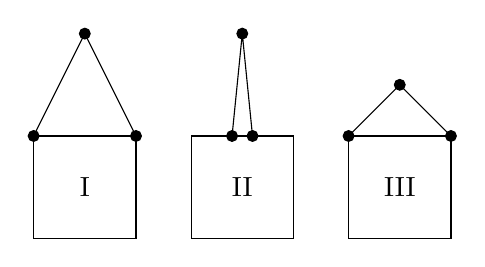
\begin{tikzpicture}
        \begin{scope}[xshift=-2cm,scale=1.3]
            \node[anchor=center] at (0,0) {I};
            \draw (-0.5,-0.5) rectangle (0.5,0.5);
            \draw[fill] (-0.5,0.5) circle (1.5pt);
            \draw[fill] (+0.5,0.5) circle (1.5pt);
            \draw[fill] (0,1.5) circle (1.5pt);
            \draw (-0.5,0.5) -- (0,1.5) -- (0.5,0.5);
        \end{scope}
        \begin{scope}[xshift=0cm,scale=1.3]
            \node[anchor=center] at (0,0) {II};
            \draw (-0.5,-0.5) rectangle (0.5,0.5);
            \draw[fill] (-0.1,0.5) circle (1.5pt);
            \draw[fill] (+0.1,0.5) circle (1.5pt);
            \draw[fill] (0,1.5) circle (1.5pt);
            \draw (-0.1,0.5) -- (0,1.5) -- (0.1,0.5);
        \end{scope}
        \begin{scope}[xshift=+2cm,scale=1.3]
            \node[anchor=center] at (0,0) {III};
            \draw (-0.5,-0.5) rectangle (0.5,0.5);
            \draw[fill] (-0.5,0.5) circle (1.5pt);
            \draw[fill] (+0.5,0.5) circle (1.5pt);
            \draw[fill] (0,1.00) circle (1.5pt);
            \draw (-0.5,0.5) -- (0,1.00) -- (0.5,0.5);
        \end{scope}
    \end{tikzpicture}
    \end{center}
    The magnitude of the tension force of the string is:
    \begin{multicols}{2}
    \begin{choices}
        \wrongchoice{least in I}
        \wrongchoice{greatest in I}
        \wrongchoice{greatest in II}
        \wrongchoice{least in III}
      \correctchoice{greatest in III}
    \end{choices}
    \end{multicols}
\end{question}
}

\element{halliday-mc}{
\begin{question}{halliday-ch12-q19}
    A uniform plank is supported by two equal \SI{120}{\newton} forces at $X$ and $Y$,
        as shown. 
    \begin{center}
    \begin{tikzpicture}
        %% Floor
        \node[anchor=north,fill,pattern=north east lines,minimum width=8cm, minimum height=0.1cm] at (0,0) {};
        \draw (-4,0) -- (4,0);
        %% Uniform Plank
        \draw[thick] (-3.5,0.5) rectangle (3.5,1.5);
        %% X and Y
        \draw[ultra thick] (-3.5,0) -- (-3.0,0.5) -- (-2.5,0) -- cycle;
        \draw[ultra thick] (+3.5,0) -- (+3.0,0.5) -- (+2.5,0) -- cycle;
        \node[anchor=south] at (-3.0,0.5) {$X$};
        \node[anchor=south] at (+3.0,0.5) {$Y$};
        %% Z
        \draw[fill] (-1,0.5) circle (1.5pt) node[anchor=south] {$Z$};
    \end{tikzpicture}
    \end{center}
    The support at $X$ is then moved to $Z$ (half-way to the plank center). 
    The supporting forces at $Y$ and $Z$ are then:
    \begin{choices}
        \wrongchoice{$F_Y=\SI{240}{\newton}$, $F_Z=\SI{120}{\newton}$}
        \wrongchoice{$F_Y=\SI{200}{\newton}$, $F_Z=\SI{40}{\newton}$}
        \wrongchoice{$F_Y=\SI{40}{\newton}$,\phantom{0}  $F_Z=\SI{200}{\newton}$}
      \correctchoice{$F_Y=\SI{80}{\newton}$,\phantom{0}  $F_Z=\SI{160}{\newton}$}
        \wrongchoice{$F_Y=\SI{160}{\newton}$, $F_Z=\SI{80}{\newton}$}
    \end{choices}
\end{question}
}

\element{halliday-mc}{
\begin{question}{halliday-ch12-q20}
    A uniform rod $AB$ is \SI{1.2}{\meter} long and weighs \SI{16}{\newton}.
    It is suspended by strings $AC$ and $BD$ as shown. 
    \begin{center}
    \begin{tikzpicture}
        %% Ceiling
        \node[anchor=south,fill,pattern=north east lines,minimum width=7cm, minimum height=0.1cm] at (0,0) {};
        \draw (-3.5,0) -- (3.5,0);
        %% Uniform Rod
        \draw[fill=white!50!black] (-3,-1) rectangle (+3,-2);
        %% Lablels
        \draw[fill] (-3,-1) circle (1.5pt) node[anchor=east] {$A$};
        \draw[fill] (+3,-1) circle (1.5pt) node[anchor=west] {$B$};
        \draw[fill] (-3,0) circle (1.5pt) node[anchor=north east] {$C$};
        \draw[fill] (+3,0) circle (1.5pt) node[anchor=north west] {$D$};
        %% Ropes
        \draw (-3,-1) -- (-3,0);
        \draw (+3,-1) -- (+3,0);
        %% E and P
        \node[draw,minimum size=0.8cm] (P) at (-1.5,-3) {$P$};
        \draw[fill] (P.north) circle (1.5pt);
        \node[anchor=south] (E) at (-1.5,-1) {$E$};
        \draw[fill] (E.south) circle (1.5pt);
        \draw (P.north) -- (E.south);
    \end{tikzpicture}
    \end{center}
    A block $P$ weighing \SI{96}{\newton} is attached at $E$,
        \SI{0.30}{\meter} from $A$. 
    The magnitude of the tension force of the string $BD$ is:
    \begin{multicols}{3}
    \begin{choices}
        \wrongchoice{\SI{8.0}{\newton}}
        \wrongchoice{\SI{24}{\newton}}
      \correctchoice{\SI{32}{\newton}}
        \wrongchoice{\SI{48}{\newton}}
        \wrongchoice{\SI{80}{\newton}}
    \end{choices}
    \end{multicols}
\end{question}
}

\element{halliday-mc}{
\begin{question}{halliday-ch12-q21}
    A \SI{5.0}{\meter} weightless strut,
        hinged to a wall, is used to support an \SI{800}{\newton} block as shown. 
    \begin{center}
    \begin{tikzpicture}
        %% Hinge
        \draw (0,0.1) arc (90:-90:0.1);
        \draw (0,0.2) arc (90:-90:0.2);
        \node[anchor=west] at (0.25,0) {hinge};
        %% Rod, 36.87 53.13
        \node[fill,minimum size=1ex,circle] (R) at (3,4) {};
        \draw[line width=4pt] (53:0.2) -- (R) node[pos=0.5,anchor=south,rotate=53] {\SI{5}{\meter}};
        %% Weight
        \node[minimum size=0.8cm,draw,anchor=center] (W) at (3cm+1ex,0) {\SI{800}{\newton}};
        \draw (W.north) -- (R.east);
        \draw (R.north) -- ++(180:3) node[pos=0.5,anchor=south] {\SI{3}{\meter}};
        %% Wall
        \node[anchor=east,fill,pattern=north east lines,minimum width=0.1cm, minimum height=6cm] at (0,2) {};
        \draw (0,-1) -- (0,5);
    \end{tikzpicture}
    \end{center}
    The horizontal and vertical components of the force of the hinge on the strut are:
    \begin{choices}
        \wrongchoice{$F_H=\SI{800}{\newton}$,\phantom{0}  $F_Y=\SI{800}{\newton}$}
      \correctchoice{$F_H=\SI{600}{\newton}$,\phantom{0}  $F_Y=\SI{800}{\newton}$}
        \wrongchoice{$F_H=\SI{800}{\newton}$,\phantom{0}  $F_Y=\SI{600}{\newton}$}
        \wrongchoice{$F_H=\SI{1200}{\newton}$,            $F_Y=\SI{800}{\newton}$}
        \wrongchoice{$F_H=\text{zero}$,\phantom{0N}       $F_Y=\SI{800}{\newton}$}
    \end{choices}
\end{question}
}

\element{halliday-mc}{
\begin{question}{halliday-ch12-q22}
    A uniform plank is \SI{6.0}{\meter} long and weighs \SI{80}{\newton}.
    It is balanced on a sawhorse at its center. 
    An additional \SI{160}{\newton} weight is now placed on the left end of the plank.
    To keep the plank balanced,
        it must be moved what distance to the left?
    \begin{multicols}{3}
    \begin{choices}
        \wrongchoice{\SI{6.0}{\meter}}
      \correctchoice{\SI{2.0}{\meter}}
        \wrongchoice{\SI{1.5}{\meter}}
        \wrongchoice{\SI{1.0}{\meter}}
        \wrongchoice{\SI{0.50}{\meter}}
    \end{choices}
    \end{multicols}
\end{question}
}

\element{halliday-mc}{
\begin{question}{halliday-ch12-q23}
    A uniform \SI{240}{\gram} meter stick can be balanced by a \SI{240}{\gram} weight placed at the \SI{100}{\centi\meter} mark if the fulcrum is placed at the point marked:
    \begin{multicols}{3}
    \begin{choices}
      \correctchoice{\SI{75}{\centi\meter}}
        \wrongchoice{\SI{60}{\centi\meter}}
        \wrongchoice{\SI{50}{\centi\meter}}
        \wrongchoice{\SI{40}{\centi\meter}}
        \wrongchoice{\SI{80}{\centi\meter}}
    \end{choices}
    \end{multicols}
\end{question}
}

\element{halliday-mc}{
\begin{questionmult}{halliday-ch12-q24}
    A ladder leans against a wall. 
    \begin{center}
    \begin{tikzpicture}
        %% Wall
        \node[anchor=east,fill,pattern=north east lines,minimum width=0.1cm, minimum height=4cm] at (0,2) {};
        \draw (0,0) -- (0,4);
        %% Floor
        \node[anchor=north,fill,pattern=north east lines,minimum width=4.2cm, minimum height=0.1cm] at (1.9,0) {};
        \draw (0,0) -- (4,0);
        %% Ladder
        \draw[line width=3pt] (0,3) -- (3,0);
    \end{tikzpicture}
    \end{center}
    If the ladder is not to slip,
        which one of the following must be true?
    \begin{choices}
        \wrongchoice{The coefficient of friction between the ladder and the wall must not be zero}
      \correctchoice{The coefficient of friction between the ladder and the floor must not be zero}
        %% questionmult
        %\wrongchoice{Both A and B}
        %\wrongchoice{Either A or B}
        %\wrongchoice{Neither A nor B}
        %\wrongchoice{ans: B}
    \end{choices}
\end{questionmult}
}

\element{halliday-mc}{
\begin{question}{halliday-ch12-q25}
    An \SI{80}{\newton} uniform plank leans against a frictionless wall as shown. 
    \begin{center}
    \begin{tikzpicture}
        %% Wall
        \node[anchor=east,fill,pattern=north east lines,minimum width=0.1cm, minimum height=5cm] at (0,2.5) {};
        \draw (0,0) -- (0,5);
        \draw[<->] (-1,0) -- (-1,4) node[pos=0.5,anchor=center,fill=white] {\SI{4}{\meter}};
        %% Floor
        \node[anchor=north,fill,pattern=north east lines,minimum width=4.2cm, minimum height=0.1cm] at (1.9,0) {};
        \draw (0,0) -- (4,0);
        \draw[<->] (0,-1) -- (3,-1) node[pos=0.5,anchor=center,fill=white] {\SI{3}{\meter}};
        %% Ladder
        \draw[line width=3pt] (0,4) -- (3,0);
        %% Point P
        \draw[fill] (3,0) circle (3pt) node[anchor=south west] {$P$};
    \end{tikzpicture}
    \end{center}
    The magnitude of the torque (about point $P$) applied to the plank by the wall is:
    \begin{multicols}{2}
    \begin{choices}
        \wrongchoice{\SI{40}{\newton\meter}}
        \wrongchoice{\SI{60}{\newton\meter}}
      \correctchoice{\SI{120}{\newton\meter}}
        \wrongchoice{\SI{160}{\newton\meter}}
        \wrongchoice{\SI{240}{\newton\meter}}
    \end{choices}
    \end{multicols}
\end{question}
}

\element{halliday-mc}{
\begin{question}{halliday-ch12-q26}
    An \SI{800}{\newton} man stands halfway up a \SI{5.0}{\meter} long ladder of negligible weight.
    The base of the ladder is \SI{3.0}{\meter} from the wall as shown. 
    \begin{center}
    \begin{tikzpicture}
        %% Wall
        \node[anchor=east,fill,pattern=north east lines,minimum width=0.1cm, minimum height=5cm] at (0,2.5) {};
        \draw (0,0) -- (0,5);
        %% Floor
        \node[anchor=north,fill,pattern=north east lines,minimum width=4.2cm, minimum height=0.1cm] at (1.9,0) {};
        \draw (0,0) -- (4,0) node[pos=0.3,anchor=south] {\SI{3}{\meter}};
        %% Ladder
        \draw[line width=3pt] (0,4) -- (3,0);
        %% Person
        \begin{scope}[yshift=2cm,xshift=1.5cm]
            \draw[thick] (0,0.25) -- (0,0.75);
            %% Legs
            \draw[thick] (0,0.25) -- (-0.25,0);
            \draw[thick] (0,0.25) -- (+0.25,0);
            %% Arms
            \draw[thick] (0,0.50) -- (-0.25,0.55);
            \draw[thick] (0,0.50) -- (+0.25,0.55);
            %% Head
            \draw[fill=white!90!black] (0,0.80) circle (0.15cm);
        \end{scope}
    \end{tikzpicture}
    \end{center}
    Assuming that the wall-ladder contact is frictionless,
        the wall pushes against the ladder with a force of magnitude:
    \begin{multicols}{3}
    \begin{choices}
        \wrongchoice{\SI{150}{\newton}}
      \correctchoice{\SI{300}{\newton}}
        \wrongchoice{\SI{400}{\newton}}
        \wrongchoice{\SI{600}{\newton}}
        \wrongchoice{\SI{800}{\newton}}
    \end{choices}
    \end{multicols}
\end{question}
}

\element{halliday-mc}{
\begin{question}{halliday-ch12-q27}
    A uniform ladder is \SI{10}{\meter} long and weighs \SI{400}{\newton}.
    It rests with its upper end against a frictionless vertical wall. 
    Its lower end rests on the ground and is prevented from slipping by a peg driven into the ground. 
    The ladder makes a \ang{30} angle with the horizontal. 
    \begin{center}
    \begin{tikzpicture}
        %% Wall
        \node[anchor=west,fill,pattern=north east lines,minimum width=0.1cm, minimum height=3.2cm] at (0,1.4) {};
        \draw (0,0) -- (0,3);
        %% Floor
        \node[anchor=north,fill,pattern=north east lines,minimum width=5.2cm, minimum height=0.1cm] at (-2.4,0) {};
        \draw (0,0) -- (-5,0);
        %% Ladder
        \draw[line width=3pt] (-4,0) -- ++(30:4.62);
        \draw[<->] (-3,0) arc (0:30:1) node[pos=0.5,anchor=west] {\ang{30}};
        %% Peg
        \draw[line width=3pt] (-4,0) -- ++(120:0.75) node[anchor=east] {peg};
    \end{tikzpicture}
    \end{center}
    The magnitude of the force exerted on the peg by the ladder is:
    \begin{multicols}{3}
    \begin{choices}
        \wrongchoice{zero}
        \wrongchoice{\SI{200}{\newton}}
        \wrongchoice{\SI{400}{\newton}}
      \correctchoice{\SI{470}{\newton}}
        \wrongchoice{\SI{670}{\newton}}
    \end{choices}
    \end{multicols}
\end{question}
}

\element{halliday-mc}{
\begin{question}{halliday-ch12-q28}
    A window washer attempts to lean a ladder against a frictionless wall. 
    He finds that the ladder slips on the ground when it is placed at an angle of less than \ang{75} to the ground but remains in place when the angle is greater than 75 ◦ . The coefficient of static friction between the ladder and the ground:
    \begin{choices}
      \correctchoice{is about 0.13}
        \wrongchoice{is about 0.27}
        \wrongchoice{is about 1.0}
        \wrongchoice{depends on the mass of the ladder}
        \wrongchoice{depends on the length of the ladder}
    \end{choices}
\end{question}
}

\newcommand{\hallidayChTwelveQTwentyNine}{
\begin{tikzpicture}
    %% Wall
    \node[anchor=west,fill,pattern=north east lines,minimum width=0.1cm,minimum height=4cm] at (1,0.5) {};
    \draw (1,-1.5) -- (1,2.5);
    %% Ball
    \draw (0,0) circle (1cm);
    \draw[fill] (0,0) circle (1.5pt);
    \node[anchor=east] at (-1,0) {\SI{600}{\newton}};
    %% string
    \draw[fill] (60:1) circle (1.5pt) node[anchor=north east] {$B$};
    \draw[fill] (60:2) circle (1.5pt) node[anchor=west,xshift=0.1cm] {$A$};
    \draw (60:1) -- (60:2);
    \draw[thick,<-] (60:2) ++(240:0.75) arc (240:200:0.75) node[anchor=south] {\ang{30}}; 
    \draw[thick,<-] (60:2) ++(270:0.75) arc (270:300:0.75); 
\end{tikzpicture}
}

\element{halliday-mc}{
\begin{question}{halliday-ch12-q29}
    The \SI{600}{\newton} ball shown is suspended on a string $AB$ and rests against a frictionless vertical wall.
    \begin{center}
        \hallidayChTwelveQTwentyNine
    \end{center}
    The string makes an angle of \ang{30} with the wall. 
    The magnitude of the tension force of the string is:
    \begin{multicols}{2}
    \begin{choices}
      \correctchoice{\SI{690}{\newton}}
        \wrongchoice{\SI{1200}{\newton}}
        \wrongchoice{\SI{2100}{\newton}}
        \wrongchoice{\SI{2400}{\newton}}
        \wrongchoice{none of the provided}
    \end{choices}
    \end{multicols}
\end{question}
}

\element{halliday-mc}{
\begin{question}{halliday-ch12-q30}
    The \SI{600}{\newton} ball shown is suspended on a string $AB$ and rests against a frictionless vertical wall.
    \begin{center}
        \hallidayChTwelveQTwentyNine
    \end{center}
    The string makes an angle of \ang{30} with the wall. 
    The ball presses against the wall with a force of mangitude:
    \begin{multicols}{3}
    \begin{choices}
        \wrongchoice{\SI{120}{\newton}}
        \wrongchoice{\SI{300}{\newton}}
      \correctchoice{\SI{350}{\newton}}
        \wrongchoice{\SI{600}{\newton}}
        \wrongchoice{\SI{690}{\newton}}
    \end{choices}
    \end{multicols}
\end{question}
}

\element{halliday-mc}{
\begin{question}{halliday-ch12-q31}
    The uniform rod shown below is held in place by the rope and wall. 
    \begin{center}
    \begin{tikzpicture}
        %% Coordinates
        \coordinate (A) at (-6,0);
        \coordinate (B) at (-3,0);
        \coordinate (C) at (0,0);
        \coordinate (E) at (0,3);
        %% Line
        \node[draw,fill=white!80!black,minimum width=6cm,minimum height=0.1cm] at (B) {};
        \draw (A) -- (D) -- (E);
        %% Nodes
        \draw[fill] (A) circle (1.5pt) node[anchor=north,yshift=-0.1cm] {$4$};
        \draw[fill] (B) circle (1.5pt) node[anchor=north,yshift=-0.1cm] {$3$};
        \draw[fill] (C) circle (1.5pt) node[anchor=north east,yshift=-0.1cm] {$2$};
        \draw[fill] (E) circle (1.5pt) node[anchor=south east] {$1$};
        %% Wall
        \node[anchor=west,fill,pattern=north east lines,minimum width=0.1cm, minimum height=5cm] at (0,1.5) {};
        \draw (0,-1) -- (0,4);
    \end{tikzpicture}
    \end{center}
    Suppose you know the weight of the rod and all dimensions. 
    Then you can solve a single equation for the force of the rope on the rod,
        provided you write expressions for the torques about the point:
    \begin{multicols}{3}
    \begin{choices}
        \wrongchoice{1}
      \correctchoice{2}
        \wrongchoice{3}
        \wrongchoice{4}
        \wrongchoice{1, 2, or 3}
    \end{choices}
    \end{multicols}
\end{question}
}

\element{halliday-mc}{
\begin{question}{halliday-ch12-q32}
    A \SI{240}{\newton} weight is hung from two ropes as shown. 
    \begin{center}
    \begin{tikzpicture}
        %% Ceiling
        \node[anchor=south,fill,pattern=north east lines,minimum width=7.2cm, minimum height=0.1cm] at (3.4,0) {};
        \draw (0,0) -- (7,0);
        %% Wall
        \node[anchor=east,fill,pattern=north east lines,minimum width=0.1cm, minimum height=4cm] at (0,-2) {};
        \draw (0,0) -- (0,-4);
        %% Nodes
        \draw[fill] (0,-2) circle (1.5pt);
        \draw[fill] (2,-2) circle (1.5pt);
        \draw[fill] (6,0) circle (1.5pt);
        \draw[thick] (0,-2) -- (2,-2) -- (6,0);
        %% angle
        \draw[<->] (3,-2) arc (0:30:1) node[pos=0.5,anchor=west] {\ang{30}};
        \draw[dashed] (2,-2) -- (3.5,-2);
        %% weight
        \node[minimum size=1cm,draw] (W) at (2,-3) {\SI{240}{\newton}};
        \draw[thick] (W.north) -- (2,-2);
    \end{tikzpicture}
    \end{center}
    The tension force of the horizontal rope has magnitude:
    \begin{multicols}{3}
    \begin{choices}
        \wrongchoice{zero}
        \wrongchoice{\SI{656}{\newton}}
        \wrongchoice{\SI{480}{\newton}}
      \correctchoice{\SI{416}{\newton}}
        \wrongchoice{\SI{176}{\newton}}
    \end{choices}
    \end{multicols}
\end{question}
}

\element{halliday-mc}{
\begin{question}{halliday-ch12-q33}
    A \SI{960}{\newton} block is suspended as shown. 
    \begin{center}
    \begin{tikzpicture}
        %% Hinge
        \draw (0,0.1) arc (90:-90:0.1);
        \draw (0,0.2) arc (90:-90:0.2);
        %% Rod, 36.87 53.13
        \node[anchor=south west] at (0.2,0) {$A$};
        \node[anchor=south west] at (4,0) {$B$};
        \draw[line width=4pt] (0.2,0) -- (4.5,0);
        %% support string
        \draw[fill] (0,3) circle (1.5pt) node[anchor=south west] {$C$};
        \draw[thick] (0,3) -- (4,0);
        %% Weight
        \node[minimum size=0.8cm,draw,anchor=center] (W) at (4,-1.5) {\SI{960}{\newton}};
        \draw (W.north) -- (4,0);
        \draw[<->] (0,-0.5) -- (4,-0.5) node[pos=0.5,anchor=center,fill=white] {\SI{4}{\meter}};
        %% Wall
        \node[anchor=east,fill,pattern=north east lines,minimum width=0.1cm, minimum height=6cm] at (0,1) {};
        \draw (0,-2) -- (0,4);
        \draw[<->] (-1,0) -- (-1,3) node[pos=0.5,anchor=center,fill=white] {\SI{3}{\meter}};
    \end{tikzpicture}
    \end{center}
    The beam $AB$ is weightless and is hinged to the wall at $A$. 
    The tension force of the cable BC has magnitude:
    \begin{multicols}{2}
    \begin{choices}
        \wrongchoice{\SI{720}{\newton}}
        \wrongchoice{\SI{1200}{\newton}}
        \wrongchoice{\SI{1280}{\newton}}
      \correctchoice{\SI{1600}{\newton}}
        \wrongchoice{none of these}
    \end{choices}
    \end{multicols}
\end{question}
}

\element{halliday-mc}{
\begin{question}{halliday-ch12-q34}
    A horizontal beam of weight $W$ is supported by a hinge and cable as shown.
    \begin{center}
    \begin{tikzpicture}
        %% Hinge
        \draw (0,0.1) arc (90:-90:0.1);
        \draw (0,0.2) arc (90:-90:0.2);
        \node[anchor=east] at (-0.15,0) {hinge};
        %% Rod, 36.87 53.13
        \draw[line width=4pt] (0.2,0) -- (4.5,0);
        \draw[thick,->] (2.25,0) -- ++(270:1.5) node[anchor=south west] {$W$};
        %% support string
        \draw[fill] (0,3) circle (1.5pt);
        \draw[thick] (0,3) -- (4,0) node[pos=0.5,anchor=south west] {cable};
        %% Wall
        \node[anchor=east,fill,pattern=north east lines,minimum width=0.1cm, minimum height=6cm] at (0,1) {};
        \draw (0,-2) -- (0,4);
    \end{tikzpicture}
    \end{center}
    The force exerted on the beam by the hinge has a vertical component that must be:
    \begin{choices}
      \correctchoice{nonzero and up}
        \wrongchoice{nonzero and down}
        \wrongchoice{nonzero but not enough information given to know whether up or down}
        \wrongchoice{zero}
        \wrongchoice{equal to $W$}
    \end{choices}
\end{question}
}

%\element{halliday-mc}{
%\begin{question}{halliday-ch12-q35}
%    A \SI{400}{\newton} uniform vertical boom is attached to the ceiling by a hinge,
%        as shown. 
%    \begin{center}
%    \begin{tikzpicture}
%        %% NOTE: jphafner
%        %% Ceiling
%        \node[anchor=east,fill,pattern=north east lines,minimum width=6cm, minimum height=0.1cm] at (0,0) {};
%        \draw (0,-2) -- (0,4);
%    \end{tikzpicture}
%    \end{center}
%    An \SI{800}{\newton} weight $W$ and a horizontal guy wire are attached to the lower end of the boom as indicated.
%    The pulley is massless and frictionless. 
%    The tension force $T$ of the horizontal guy wire has magnitude:
%    \begin{multicols}{3}
%    \begin{choices}
%        \wrongchoice{\SI{340}{\newton}}
%      \correctchoice{\SI{400}{\newton}}
%        \wrongchoice{\SI{690}{\newton}}
%        \wrongchoice{\SI{800}{\newton}}
%        \wrongchoice{\SI{1200}{\newton}}
%    \end{choices}
%    \end{multicols}
%\end{question}
%}

\element{halliday-mc}{
\begin{question}{halliday-ch12-q36}
    A picture is to be hung from the ceiling by means of two wires. 
    \begin{center}
    \begin{tikzpicture}
        %% Ceiling
        \node[anchor=south,fill,pattern=north east lines,minimum width=3cm, minimum height=0.1cm] at (0,0) {};
        \draw (-1.5,0) -- (1.5,0);
        %% Block
        \draw[very thick,fill=white!90!black] (-1,-1) rectangle (1,-2);
        \draw[fill] (0,-1.5) circle (1pt) node[anchor=west] {cm};
        %% strings
        \draw (-1,0) -- (-1,-1) node[pos=0.5,anchor=east] {$A$};
        \draw (+1,0) -- (+1,-1) node[pos=0.5,anchor=west] {$B$};
        %% Label
        \node[anchor=center] at (0,-0.5) {I};
    \end{tikzpicture}
    \hspace{2\baselineskip}
    \begin{tikzpicture}
        %% Ceiling
        \node[anchor=south,fill,pattern=north east lines,minimum width=3cm, minimum height=0.1cm] at (0,0) {};
        \draw (-1.5,0) -- (1.5,0);
        %% Block
        \draw[very thick,fill=white!90!black] (-1,-1) rectangle (1,-2);
        \draw[fill] (0,-1.5) circle (1pt) node[anchor=west] {cm};
        %% strings
        \draw (-0.5,0) -- (-0.5,-1) node[pos=0.5,anchor=east] {$A$};
        \draw (+1,0) -- (+1,-1) node[pos=0.5,anchor=west] {$B$};
        %% Label
        \node[anchor=center] at (0,-0.5) {II};
    \end{tikzpicture}

    \vspace{\baselineskip}
    \begin{tikzpicture}
        %% Ceiling
        \node[anchor=south,fill,pattern=north east lines,minimum width=3cm, minimum height=0.1cm] at (0,0) {};
        \draw (-1.5,0) -- (1.5,0);
        %% Block
        \draw[very thick,fill=white!90!black] (-1,-1) rectangle (1,-2);
        \draw[fill] (0,-1.5) circle (1pt) node[anchor=west] {cm};
        %% strings
        \draw (-1,0) -- (-1,-1) node[pos=0.5,anchor=east] {$A$};
        \draw (+0.5,0) -- (+0.5,-1) node[pos=0.5,anchor=west] {$B$};
        %% Label
        \node[anchor=center] at (0,-0.5) {III};
    \end{tikzpicture}
    \end{center}
    Order the following arrangements of the wires according to the tension force of wire $B$,
        from least to greatest.
    \begin{multicols}{2}
    \begin{choices}
        \wrongchoice{I, II, III}
        \wrongchoice{III, II, I}
        \wrongchoice{I and II tie, then III}
      \correctchoice{II, I, III}
        \wrongchoice{all tie}
    \end{choices}
    \end{multicols}
\end{question}
}

\element{halliday-mc}{
\begin{question}{halliday-ch12-q37}
    The pull $P$ is just sufficient to keep the \SI{14}{\newton} block and the weightless pulleys in equilibrium as shown.
    \begin{center}
    \begin{tikzpicture}
        %% Ceiling
        \node[anchor=south,fill,pattern=north east lines,minimum width=3cm, minimum height=0.1cm] at (0.5,0) {};
        \draw (-1,0) -- (2,0);
        \draw[fill] (0,0) circle (1.5pt);
        %% top pulley
        \draw[fill=white!90!black] (0,-1.5) circle (0.5);
        \draw[fill] (0,-1.5) circle (1.5pt);
        \draw (0,0) -- (0,-1.5) node[pos=0.25,anchor=east] {$T$};
        \draw (-0.5,-1.5) -- (-0.5,-6);
        %% middle pulley
        \draw[fill=white!90!black] (0.5,-3) circle (0.5);
        \draw[fill] (0.5,-3) circle (1.5pt);
        \draw (+0.5,-1.5) -- (+0.5,-3);
        \draw (0,-3) -- (0,-6);
        %% botttom pulley
        \draw[fill=white!90!black] (1,-4.5) circle (0.5);
        \draw[fill] (1,-4.5) circle (1.5pt);
        \draw (1,-3) -- (1,-4.5);
        \draw (0.5,-4.5) -- (0.5,-6);
        \draw[->] (1.5,-4.5) -- (1.5,-6) node[pos=0.75,anchor=west] {$P$};
        %% 14 N Weight (typo)
        \node[fill=white!90!black,anchor=north,draw,minimum width=2cm,minimum height=1cm] (W) at (0,-6) {\SI{14}{\newton}};
    \end{tikzpicture}
    \end{center}
    The magnitude $T$ of the tension force of the upper cable is:
    \begin{multicols}{3}
    \begin{choices}
        \wrongchoice{\SI{14}{\newton}}
        \wrongchoice{\SI{28}{\newton}}
      \correctchoice{\SI{16}{\newton}}
        \wrongchoice{\SI{9.33}{\newton}}
        \wrongchoice{\SI{18.7}{\newton}}
    \end{choices}
    \end{multicols}
\end{question}
}

\element{halliday-mc}{
\begin{question}{halliday-ch12-q38}
    The ideal mechanical advantage
        (i.e. the ratio of the weight $W$ to the pull $P$ for equilibrium)
        of the combination of pulleys shown is:
    \begin{center}
    \begin{tikzpicture}
        %% Ceiling
        \node[anchor=south,fill,pattern=north east lines,minimum width=4cm, minimum height=0.1cm] at (1,0) {};
        \draw (-1,0) -- (3,0);
        \draw[fill] (0,0) circle (1.5pt);
        %% top pulley
        \draw[fill=white!90!black] (0,-1.5) circle (0.5);
        \draw[fill] (0,-1.5) circle (1.5pt);
        \draw (0,0) -- (0,-1.5);
        \draw[->] (-0.5,-1.5) -- (-0.5,-3) node[pos=0.75,anchor=east] {$P$};
        %% middle pulley
        \draw[fill=white!90!black] (1,-3) circle (0.5);
        \draw[fill] (1,-3) circle (1.5pt);
        \draw (0.5,-3) -- (0.5,-1.5);
        \draw (1.5,-3) -- (1.5,0);
        \draw[fill] (1.5,0) circle (1.5pt);
        %% bottom pulley
        \draw[fill=white!90!black] (1.5,-4.5) circle (0.5);
        \draw[fill] (1.5,-4.5) circle (1.5pt);
        \draw (1,-4.5) -- (1,-3);
        \draw (2,-4.5) -- (2,0);
        \draw[fill] (2,0) circle (1.5pt);
        \draw (1.5,-4.5) -- (1.5,-6);
        %% Weight
        \node[fill=white!90!black,anchor=north,draw,minimum size=1cm] (W) at (1.5,-6) {$W$};
    \end{tikzpicture}
    \end{center}
    \begin{multicols}{3}
    \begin{choices}
        \wrongchoice{\num{1}}
        \wrongchoice{\num{2}}
        \wrongchoice{\num{3}}
      \correctchoice{\num{4}}
        \wrongchoice{\num{5}}
    \end{choices}
    \end{multicols}
\end{question}
}

\element{halliday-mc}{
\begin{question}{halliday-ch12-q39}
    Stress can be measured in:
    \begin{choices}
      \correctchoice{newton per meter squared (\si{\newton\per\meter\squared})}
        \wrongchoice{newton meter squared (\si{\newton\meter\squared})}
        \wrongchoice{newton per meter (\si{\newton\meter})}
        \wrongchoice{newton meter (\si{\newton\meter})}
        \wrongchoice{none of the provided (it is unitless)}
    \end{choices}
\end{question}
}

\element{halliday-mc}{
\begin{question}{halliday-ch12-q40}
    Strain can be measured in:
    \begin{choices}
        \wrongchoice{newton per meter squared (\si{\newton\per\meter\squared})}
        \wrongchoice{newton meter squared (\si{\newton\meter\squared})}
        \wrongchoice{newton per meter (\si{\newton\meter})}
        \wrongchoice{newton meter (\si{\newton\meter})}
      \correctchoice{none of the provided (it is unitless)}
    \end{choices}
\end{question}
}

\element{halliday-mc}{
\begin{question}{halliday-ch12-q41}
    Young's modulus can be correctly given in:
    \begin{choices}
        \wrongchoice{newton meter (\si{\newton\meter})}
      \correctchoice{newton per meter squared (\si{\newton\per\meter\squared})}
        \wrongchoice{newton meter per second (\si{\newton\meter\per\second})}
        \wrongchoice{newton per meter (\si{\newton\meter})}
        \wrongchoice{joule (\si{\joule})}
    \end{choices}
\end{question}
}

\element{halliday-mc}{
\begin{question}{halliday-ch12-q42}
    Young's modulus is a proportionality constant that relates the force per unit area applied perpendicularly at the surface of an object to:
    \begin{choices}
        \wrongchoice{the shear}
        \wrongchoice{the fractional change in volume}
      \correctchoice{the fractional change in length}
        \wrongchoice{the pressure}
        \wrongchoice{the spring constant}
    \end{choices}
\end{question}
}

\element{halliday-mc}{
\begin{question}{halliday-ch12-q43}
    Young's modulus can be used to calculate the strain for a stress that is:
    \begin{choices}
        \wrongchoice{just below the ultimate strength}
        \wrongchoice{just above the ultimate strength}
      \correctchoice{well below the yield strength}
        \wrongchoice{well above the yield strength}
        \wrongchoice{none of the provided}
    \end{choices}
\end{question}
}

\element{halliday-mc}{
\begin{question}{halliday-ch12-q44}
    The ultimate strength of a sample is the stress at which the sample:
    \begin{choices}
        \wrongchoice{returns to its original shape when the stress is removed}
        \wrongchoice{remains underwater}
      \correctchoice{breaks}
        \wrongchoice{bends \ang{180}}
        \wrongchoice{does none of these}
    \end{choices}
\end{question}
}

\element{halliday-mc}{
\begin{question}{halliday-ch12-q45}
    A certain wire stretches \SI{0.90}{\centi\meter} when outward forces with magnitude $F$ are applied to each end. 
    The same forces are applied to a wire of the same material but with three times the diameter and three times the length.
    The second wire stretches:
    \begin{multicols}{3}
    \begin{choices}
        \wrongchoice{\SI{0.10}{\centi\meter}}
      \correctchoice{\SI{0.30}{\centi\meter}}
        \wrongchoice{\SI{0.90}{\centi\meter}}
        \wrongchoice{\SI{2.7}{\centi\meter}}
        \wrongchoice{\SI{8.1}{\centi\meter}}
    \end{choices}
    \end{multicols}
\end{question}
}

\element{halliday-mc}{
\begin{question}{halliday-ch12-q46}
    A force of \SI{5000}{\newton} is applied outwardly to each end of a \SI{5.0}{\meter} long rod with a radius of \SI{34.0}{\centi\meter} and a Young's modulus of \SI{125e8}{\newton\per\meter\squared}.
    The elongation of the rod is:
    \begin{multicols}{2}
    \begin{choices}
        \wrongchoice{\SI{0.0020}{\milli\meter}}
        \wrongchoice{\SI{0.0040}{\milli\meter}}
        \wrongchoice{\SI{0.14}{\milli\meter}}
      \correctchoice{\SI{0.55}{\milli\meter}}
        \wrongchoice{\SI{1.42}{\milli\meter}}
    \end{choices}
    \end{multicols}
\end{question}
}

\element{halliday-mc}{
\begin{question}{halliday-ch12-q47}
    A \SI{4.0}{\meter} long steel beam with a cross-sectional area of \SI{1.0e-2}{\meter\squared} and a Young's modulus of \SI{2.0e11}{\newton\per\meter\squared} is wedged horizontally between two vertical walls. 
    In order to wedge the beam, it is compressed by \SI{0.020}{\milli\meter}. 
    If the coefficient of static friction between the beam and the walls is \num{0.70} the maximum mass (including its own) it can bear without slipping is:
    \begin{multicols}{3}
    \begin{choices}
        \wrongchoice{zero}
        \wrongchoice{\SI{3.6}{\kilo\gram}}
        \wrongchoice{\SI{36}{\kilo\gram}}
        \wrongchoice{\SI{71}{\kilo\gram}}
      \correctchoice{\SI{710}{\kilo\gram}}
    \end{choices}
    \end{multicols}
\end{question}
}

\element{halliday-mc}{
\begin{question}{halliday-ch12-q48}
    Two supports, made of the same material and initially of equal length, are \SI{2.0}{\meter} apart. 
    A stiff board with a length of \SI{4.0}{\meter} and a mass of \SI{10}{\kilo\gram} is placed on the supports,
        with one support at the left end and the other at the midpoint. 
    A block is placed on the board a distance of \SI{0.50}{\meter} from the left end. 
    As a result the board is horizontal. 
    The mass of the block is:
    \begin{multicols}{3}
    \begin{choices}
        \wrongchoice{zero}
        \wrongchoice{\SI{2.3}{\kilo\gram}}
        \wrongchoice{\SI{6.6}{\kilo\gram}}
        \wrongchoice{\SI{10}{\kilo\gram}}
      \correctchoice{\SI{20}{\kilo\gram}}
    \end{choices}
    \end{multicols}
\end{question}
}

\element{halliday-mc}{
\begin{question}{halliday-ch12-q49}
    The bulk modulus is a proportionality constant that relates the pressure acting on an object to:
    \begin{choices}
        \wrongchoice{the shear}
      \correctchoice{the fractional change in volume}
        \wrongchoice{the fractional change in length}
        \wrongchoice{Young’s modulus}
        \wrongchoice{the spring constant}
    \end{choices}
\end{question}
}

\element{halliday-mc}{
\begin{question}{halliday-ch12-q50}
    A cube with edges exactly \SI{2}{\centi\meter} long is made of material with a bulk modulus of \SI{3.5e9}{\newton\per\meter\squared}.
    When it is subjected to a pressure of \SI{3.0e5}{\pascal} its volume is:
    \begin{multicols}{2}
    \begin{choices}
        \wrongchoice{\SI{7.31}{\centi\meter\cubed}}
      \correctchoice{\SI{7.99931}{\centi\meter\cubed}}
        \wrongchoice{\SI{8.00069}{\centi\meter\cubed}}
        \wrongchoice{\SI{8.69}{\centi\meter\cubed}}
        \wrongchoice{none of the provided}
    \end{choices}
    \end{multicols}
\end{question}
}

\element{halliday-mc}{
\begin{question}{halliday-ch12-q51}
    A cube with \SI{2.0}{\centi\meter} sides is made of material with a bulk modulus of \SI{4.7e5}{\newton\per\meter}.
    When it is subjected to a pressure of \SI{2.0e5}{\pascal} the length of its any of its sides is:
    \begin{multicols}{2}
    \begin{choices}
        \wrongchoice{\SI{0.85}{\centi\meter}}
        \wrongchoice{\SI{1.15}{\centi\meter}}
      \correctchoice{\SI{1.66}{\centi\meter}}
        \wrongchoice{\SI{2.0}{\centi\meter}}
        \wrongchoice{none of the provided}
    \end{choices}
    \end{multicols}
\end{question}
}

\element{halliday-mc}{
\begin{question}{halliday-ch12-q52}
    To shear a cube-shaped object,
        forces of equal magnitude and opposite directions might be applied:
    \begin{choices}
        \wrongchoice{to opposite faces, perpendicular to the faces}
      \correctchoice{to opposite faces, parallel to the faces}
        \wrongchoice{to adjacent faces, perpendicular to the faces}
        \wrongchoice{to adjacent faces, neither parallel or perpendicular to the faces}
        \wrongchoice{to a single face, in any direction}
    \end{choices}
\end{question}
}

\element{halliday-mc}{
\begin{question}{halliday-ch12-q53}
    A shearing force of \SI{50}{\newton} is applied to an aluminum rod with a length of \SI{10}{\meter},
        a cross-sectional area of \SI{1.0e-5}{\meter\squared},
        and a shear modulus of \SI{2.5e10}{\newton\per\meter}. 
    As a result the rod is sheared through a distance of:
    \begin{multicols}{3}
    \begin{choices}
        \wrongchoice{zero}
      \correctchoice{\SI{1.9}{\milli\meter}}
        \wrongchoice{\SI{1.9}{\centi\meter}}
        \wrongchoice{\SI{19}{\centi\meter}}
        \wrongchoice{\SI{1.9}{\meter}}
    \end{choices}
    \end{multicols}
\end{question}
}


\endinput


